\documentclass[12pt,a4paper, twosite]{article}
\usepackage[spanish]{babel}
\usepackage[utf8]{inputenc}
\usepackage[T1]{fontenc}
\usepackage{graphicx}
\usepackage{grffile}
\usepackage{longtable}
\usepackage{wrapfig}
\usepackage{rotating}
\usepackage[normalem]{ulem}
\usepackage{amsmath}
\usepackage{textcomp}
\usepackage{amssymb}
\usepackage{capt-of}
\usepackage{hyperref}
\usepackage[left=2.00cm, right=2.50cm, top=2.50cm, bottom=2.00cm]{geometry}
\usepackage{fancyhdr}
\fancyhead[RO,LE]{\thepage}
\fancyhead[LO]{\emph{\uppercase{\leftmark}}}
\fancyfoot{}
\renewcommand{\headrulewidth}{1.0pt}
\pagestyle{fancy}
\date{\today}
\author{Gaston Valdez \\ gaston.cb.90@gmail.com}
\title{Telemetría y sistema de posicionamiento de antena para interferometría \\ Documento de arquitectura y diseño detallado  	}
\hypersetup{
	pdfborder={0 0 0},
	pdfauthor={Gastón Valdez},
	pdftitle={Reqerimientos de ingenieria de software},
	pdfkeywords={Requerimientos, posicionador de antena},
	pdfsubject={hola mundo},
	pdfcreator={Emacs 26.2 (Org mode 9.1.9)}, 
	pdflang={Spanish}
}
\begin{document}
\begin{titlepage}
	\maketitle
\end{titlepage}	
	\tableofcontents
	
	\newpage
	
\section{Introducción}
\label{sec:org60390fa}


	

\subsection{Propósito}
\label{sec:org434c3ef}
\begin{enumerate}
	\item El documento describe la arquitectura de software que se desarrolla para el sistema de posicionamiento perteneciente al interferómetro MIA (\ref{ref:MIA}) y estaciones terrenas del IAR.  
	\item Está dirigido a desarrolladores de software embebido pertenecientes al IAR.
	
\end{enumerate}	
	
	
	\subsection{Ámbito del sistema}
	\label{sec:org12e44a1}
	\begin{enumerate}
		\item El equipo se denomina ROT\_IAR. 
	\end{enumerate}
	\subsection{Definiciones, Acrónimos y Abreviaturas}
	\label{sec:orgb158e36}
	\begin{itemize}
		\item IAR: Instituto Argentino de Radiastronomía.
		\item MIA: milimmeter instrument array.
		\item FIUBA: Facultad de ingeniería de la Universidad de Buenos Aires.  		
		\item SBC: Single Board Computer. 
		\item WBS: Work Breakdown Structure o estructura de desglose de trabajo.  	
	\end{itemize}
	
	\subsection{Referencias}
	\label{sec:org62711e0}
	\begin{enumerate}
		\item  \label{ref:MIA}proyecto MIA: https://www.iar.unlp.edu.ar/slider/observatorio/
		\item \label{ref:cese} Plan de trabajo CESE.
		\item \label{ref:ptr} IAR-OBS-MIA-REQ-R05 (documento interno).
		\item \label{ref:ids_1} IdS\_Gaston\_Valdez\_TP1 
		\item \label{ref:ids_2} IdS\_Gaston\_Valdez\_TP2 
		
	\end{enumerate}
	
	\subsection{Visión general del documento}
	\label{sec:orgdaca22c}
	\begin{enumerate}
		
		
	\item El documento se escribe siguiendo el estandar IEEE-std 1830 exigido por la cátedra de Ingeniería de Software perteneciente a la carrera de especialización de sistemas embebidos de FIUBA. 
%	\item Se usan los patrones para el primer entregable al IAR. 
	\end{enumerate}
	
	\section{Arquitectura}
	\label{sec:orgc1c4017}
	Se presenta la arquitectura de software correspondiente al dispositivo ROT\_IAR (ver \ref{ref:cese}). Los patrones arquitectónicos de este dispositivo se enumeran a continuación:  
	\begin{enumerate}
		\item Arquitectura cliente-servidor  
		\item Patrón observar y reaccionar (leer sensores y manejo de GPIO)
		\item Segmentación de proceso (lectura de encoders) 
	\end{enumerate}
	
	\subsection{Arquitectura cliente-servidor}
	La arquitectura cliente servidor se muestra en la figura \ref{fig:arq-cl-s}. Cada bloque dentro del dispositivo ROT\_IAR presentan distintos patrones de arquitectura que se muestran en el presente informe. El bloque correspondiente a la interfaz servidor no se muestra en el presente documento. El bloque correspondiente al control se trata en la etapa 4 del WBS (\ref{ref:cese}). 
	\begin{figure}[h!]
		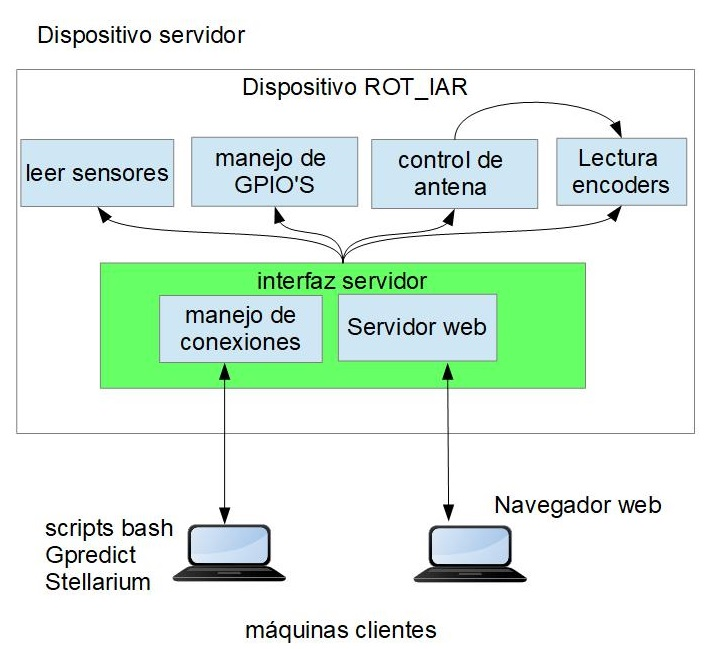
\includegraphics{arqClienteServidor.jpg} 
		\caption{Arquitectura cliente servidor del sistema ROT\_IAR} 
		\label{fig:arq-cl-s}
	\end{figure}
	
	
	\subsection{Leer sensores y manejo de GPIO'S} 
	\label{sec:orga40b0ee}
%	patron obs y reaccionar 
	La función del bloque leer sensores es realizar la lectura de temperatura, humedad y velocidad del viento. A partir de estos parámetros determina que la antena debe realizar un movimiento hacia el punto de equilibrio mecánico.El diagrama de arquitectura se muestra en la figura \ref{fig:leer}.  
	La función del bloque manejo de GPIO's es seleccionar el puerto que debe prenderse o apagarse. Su esquema de arquitectura se muestra en la figura \ref{fig:gpios}. 
	\begin{figure}[!]
	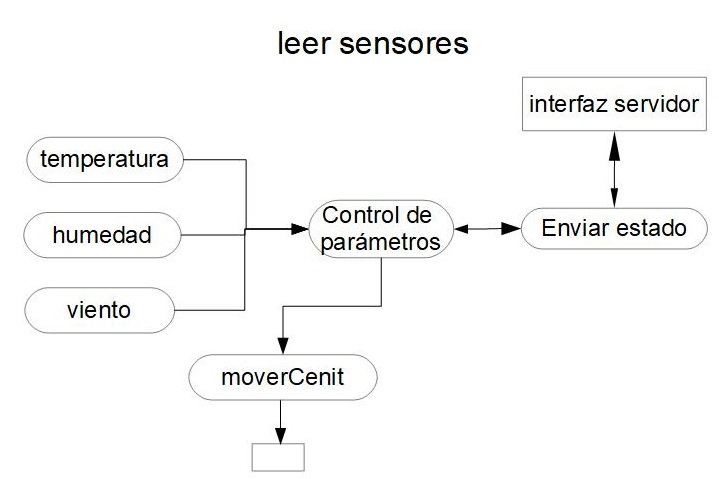
\includegraphics{leerEncoders.jpg} 
	\caption{Patrón observar y reaccionar para leer sensores} 
	\label{fig:leer}
	\end{figure}
	
	\begin{figure}[!]
		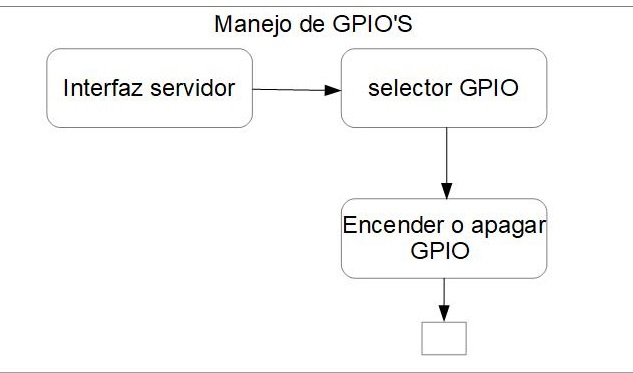
\includegraphics[trim={1cm 0.3cm 0.5cm 0.2cm},clip]{manejoGPIOS.jpg} 
		\caption{Patrón observar y reaccionar para leer sensores} 
		\label{fig:gpios}
	\end{figure}
	
	\subsection{Leer encoders}
	\label{sec:org5ca5790}
% proceso de transformación 	
	Este bloque debe realizar la lectura de los encoders adosados mecánicamente a la antena, y debe realizar la transformación correspondiente al protocolo de los programas Stellarium, Gpredict, y los script bash que pertenecen a la institución. El diagrama de arquitectura se muestra en la figura \ref{fig:lectenc}.
	\begin{figure}[h!]
	\includegraphics{lectenc.jpg} 
	\caption{Patrón observar y reaccionar para leer sensores} 
	\label{fig:lectenc}
\end{figure}
	
	\subsection{Diseños de arquitectura futuros}
	\label{sec:org33cfcdb}
% patrón arquitectónico del control 
% patrón arquitectónico de la interfaz del servidor 
\begin{enumerate}
\item Patrón arquitectónico de la interfaz de servidor. 
\item Patrón arquitectónico del control de antena. 

\end{enumerate}		
	
	

\end{document}